\documentclass[a4paper,12pt]{article}

\usepackage{cite}
\usepackage{amsmath,amssymb,amsfonts}
\usepackage{algorithmic}
\usepackage{graphicx}
\usepackage{textcomp}
\usepackage{xcolor}
\usepackage{booktabs}
\usepackage{url}
\def\BibTeX{{\rm B\kern-.05em{\sc i\kern-.025em b}\kern-.08em
    T\kern-.1667em\lower.7ex\hbox{E}\kern-.125emX}}
\begin{document}

\title{Assignment 2 : Clustering %\\
%{\footnotesize \textsuperscript{*}Note: Sub-titles are not captured for https://ieeexplore.ieee.org  and
%should not be used}
%\thanks{Identify applicable funding agency here. If none, delete this.}
}

\author{Renjiro Owen\\
\textit{Victoria University Wellington}\\
Wellington, New Zealand\\
owenrenj@myvuw.ac.nz}

\maketitle
\newpage
\section{K-means}

Figure~\ref{fig:kmeans3} shows the result of applying the K-means clustering algorithm with $K=3$. The data was tested with $K \in {2,3,4,5}$, and $K=3$ was selected because it best matches the three main groups visible in the data. Although the three clusters are generally identified, the salient groups are not completely separated as intended, with some points from the second group being incorrectly assigned to the first cluster. This occurs because K-means assigns points based on their distance to the cluster centroids and assumes that clusters are relatively spherical; consequently, it performs well for the two approximately circular groups but struggles with the elongated and slightly scattered structure of the second group. In particular, the dense points on the right side of the second group pull its centroid towards the right, while some points on its left side are closer to the first centroid and are therefore assigned to the first cluster. Thus, the result demonstrates a limitation of K-means when the underlying clusters have different shapes and densities.

\begin{figure}
	\centering
	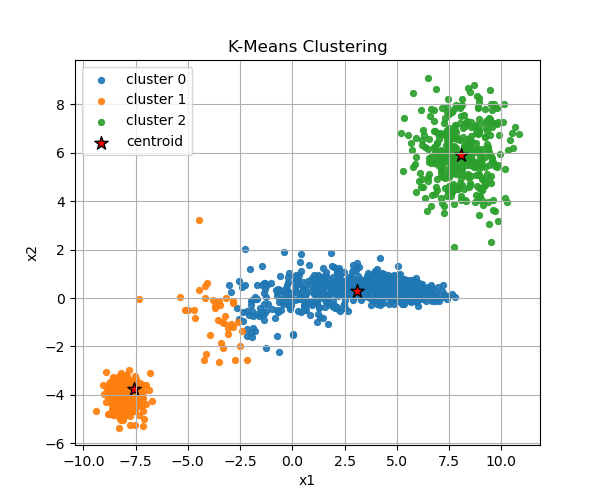
\includegraphics[width=0.8\textwidth]{../../Kmeans3Clustering.png}
	\caption{K-means clustering with $K=3$.}
	\label{fig:kmeans3}
\end{figure}

Another reasonable choice is $K=4$, as shown in Figure~\ref{fig:kmeans4}. By splitting the second group into two clusters, this result almost resolves the main issue observed with $K=3$, where some points from the second group were incorrectly assigned to the first cluster. The separation is still reasonable because the original second group contains two visibly different regions: the points on the left are more scattered, while the points on the right form a denser group. Therefore, the additional cluster can be interpreted as capturing the difference in density within the original group rather than being an entirely arbitrary split. Overall, $K=4$ provides a reasonable representation of the visible structure of the data, although the separation is primarily driven by the density and spatial distribution of the points.

\begin{figure}
	\centering
	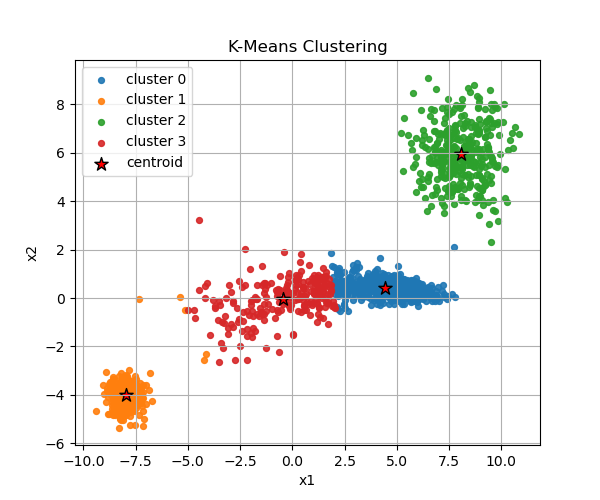
\includegraphics[width=0.8\textwidth]{../../Kmeans4Clustering.png}
	\caption{K-means clustering with $K=3$.}
	\label{fig:kmeans4}
\end{figure}

\section{DBSCAN}

\subsection{Three-cluster clustering with minimal noise}

\begin{figure}
	\centering
	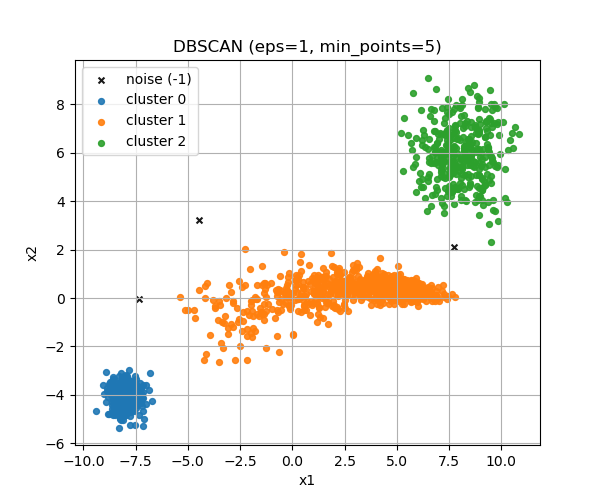
\includegraphics[width=0.8\textwidth]{../../DBScan(1,5)Clustering.png}
	\caption{K-means clustering with $K=4$.}
	\label{fig:dbscan15}
\end{figure}
Figure~\ref{fig:dbscan15} shows the DBSCAN clustering result using (EPS=1) and (MIN POINTS=5). With these settings, the data is divided into three clusters with only three points identified as noise, including isolated points on the left, between the second and third groups, and in the upper region. These settings work well because an (\text{EPS}) of 1 is large enough to connect points within the three main groups while remaining small enough to avoid merging the nearby first and second groups. Increasing (\text{EPS}) further can assign the three noise points to existing clusters, but it also increases the risk of merging the first and second groups because they are relatively close to each other.

\subsection{Clustering Based on the Densest Cores}

\begin{figure}
	\centering
	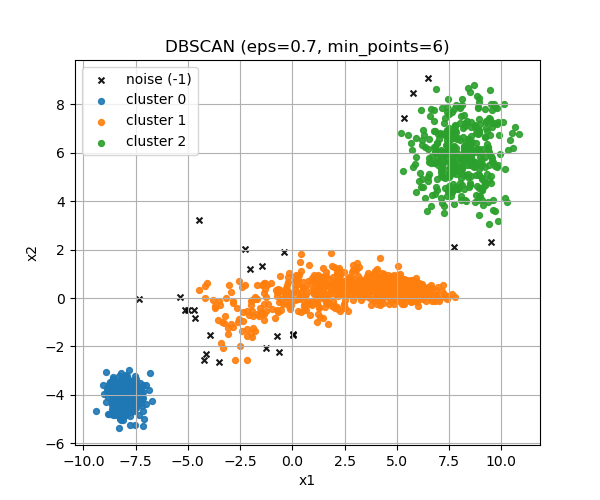
\includegraphics[width=0.8\textwidth]{../../DBScan(0.7,6)Clustering.png}
	\caption{DBSCAN clustering with EPS = 0.7 and MIN\_POINTS = 6.}
	\label{fig:dbscan076}
\end{figure}

\begin{figure}
	\centering
	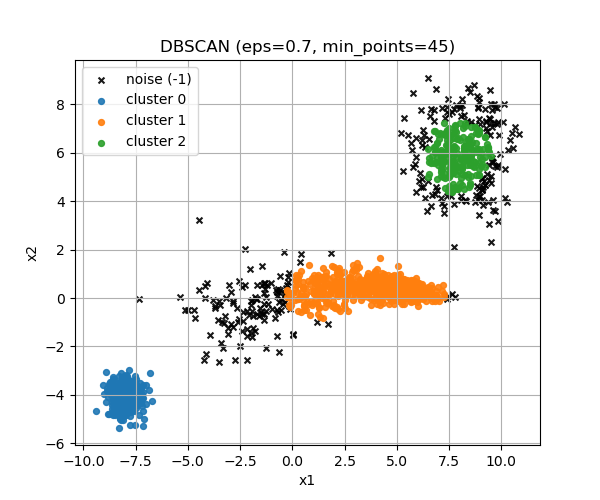
\includegraphics[width=0.8\textwidth]{../../DBScan(0.7,45)Clustering.png}
	\caption{DBSCAN clustering with EPS = 0.7 and MIN\_POINTS = 45.}
	\label{fig:dbscan0745}
\end{figure}
Figure~\ref{fig:dbscan076} shows the DBSCAN result using (EPS=0.7) and (MIN POINTS=6). These settings keep the three main groups separated while classifying several of the more scattered points as noise, which favours the denser core regions of each cluster. This occurs because the smaller (\text{EPS}) reduces the neighbourhood radius while the higher (\text{MIN POINTS}) requires more neighbouring points for a region to be considered dense. As (\text{MIN POINTS}) is increased further, DBSCAN becomes more selective about density; for example, with (\text{MIN POINTS}=45) shown in the Figure~\ref{fig:dbscan0745}, almost all of the data form the less-dense second group identified by K-means with (K=4) is classified as noise.


\section{Statement}

I declare that this assignment is my own work. The implementation, experimentation, model training, and evaluation were completed by me. Artificial intelligence Chatgpt\cite{chatgpt2026} were used only for language assistance during the preparation of this report.

\bibliographystyle{IEEEtran}   % or plain, unsrt, apalike, etc.
\bibliography{references}

\end{document}
